\documentclass[11pt]{article}
\pagestyle{plain}
\usepackage[margin=1in]{geometry}
\usepackage{amsmath,amssymb,amsthm,booktabs}
\usepackage[T1]{fontenc}
\usepackage[utf8]{inputenc}
\usepackage{lmodern}
\usepackage{graphicx}
\usepackage[hyphens]{url}
\usepackage[colorlinks=true,linkcolor=blue,citecolor=blue,urlcolor=blue]{hyperref}
\newtheorem{theorem}{Theorem}[section]
\newtheorem{lemma}[theorem]{Lemma}
\newtheorem{proposition}[theorem]{Proposition}
\theoremstyle{definition}
\newtheorem{definition}[theorem]{Definition}
\newcommand{\Z}{\mathbb Z}
\newcommand{\F}{\mathbb F}
\newcommand{\GL}{\operatorname{GL}}
\newcommand{\Aut}{\operatorname{Aut}}
\newcommand{\ord}{\operatorname{ord}}
\newcommand{\ang}[1]{\langle #1\rangle}
\newcommand{\tor}[1]{\{4,4\}_{(#1,0)}}
\setlength{\emergencystretch}{2em}
\raggedbottom
\title{Existence of locally toroidal regular 4-polytopes}
\author{P. Graham\\ \small\url{https://orcid.org/0009-0007-8493-1505}}
\date{October 24, 2026}
\hypersetup{pdfauthor={P. Graham},pdftitle={Existence of locally toroidal regular 4-polytopes}}
\begin{document}
\maketitle
\begingroup
\renewcommand{\thefootnote}{}
\footnotetext{The proofs, the Lean formalization and the text were produced by AI models (from OpenAI and Anthropic), working under the author's direction.}
\endgroup
\begin{abstract}
We prove the existence half of Schulte--Weiss Problem 16 (2006) and
McMullen--Schulte Conjecture 10C7 (2002): the universal regular
4-polytope $\{\tor{s},\tor{u}\}$ exists for every pair of distinct odd
integers $s,u\geq3$, with no coprimality assumption. Here $\tor{s}$ is the
quotient of the square tessellation by $s\Z^2$. Finiteness and group
classification remain open. The proof constructs four matrices over a
finite field of characteristic two whose local subgroups are isomorphic
to the prescribed toroidal groups. A commutator obstruction shows that
these subgroups meet exactly in the subgroup on their two shared
generators; this equality lifts to the universal presentation. The group
theorem, the geometric identification of the toroidal maps, and the
construction and universality of the resulting abstract polytope are
formalized in Lean.
\end{abstract}

\section{Introduction}
We prove existence for an exceptional family in the classification of
locally toroidal regular 4-polytopes. For an integer $p\geq3$, write
$\tor{p}$ for the square tessellation modulo the translation lattice
$p\Z^2$. Its vertices are the points of $(\Z/p\Z)^2$, with the edges and
squares inherited from the unit square grid. For example, $\tor{3}$ has
nine vertices and nine square faces. A regular 4-polytope is
\emph{locally toroidal} here when both its facets and its vertex-figures
are such toroidal maps. The double-brace notation, for example
\[
                         \{\tor{3},\tor{5}\},
\]
denotes the universal regular polytope with the indicated facets and
vertex-figures: it covers every regular polytope with those local types.
The Schläfli type records the polygon sizes of rank-two sections;
type $\{4,4,4\}$ means that all three kinds are squares.

\begin{theorem}\label{thm:main}
For every pair of distinct odd integers $s,u\geq3$, the universal regular
4-polytope
\[
                 \{\tor{s},\tor{u}\}
\]
exists. It has Schläfli type $\{4,4,4\}$, facets isomorphic to $\tor{s}$,
and vertex-figures isomorphic to $\tor{u}$.
\end{theorem}

McMullen and Schulte recorded the finite universal example with periods
$(3,5)$ and its dual \cite[pp.~375--376]{ARP}. Here we establish existence
for every pair of distinct odd periods, including pairs with common
factors. We reuse Coxeter and Moser's toroidal presentations and
McMullen and Schulte's reconstruction of regular polytopes from string
C-groups (Definition~\ref{def:string}). The hardest new step is proving that the facet and vertex-figure
groups, with independently prescribed periods, meet exactly in their
common dihedral subgroup (Proposition~\ref{prop:intersection}). Realizing
the two local maps separately does not establish this equality; the new
matrix commutator argument proves it without a coprimality assumption.

This is the existence half of Schulte--Weiss Problem 16
\cite[Problem 16]{SW} and McMullen--Schulte's 2002 Conjecture 10C7
\cite[p.~376]{ARP}. Finiteness and group classification remain open.
There is no gcd restriction: pairs such as $(3,9)$, $(9,15)$ and $(15,45)$
are included. Figure~\ref{fig:local-maps} shows the local maps for $(3,9)$.
The theorem does not assert finiteness or infiniteness of
the universal polytope for any pair. In particular, the finite matrix
group used in the proof is a quotient of the universal polytope's
automorphism group. A finite quotient does not decide finiteness of the
universal member.

Peter McMullen and Egon Schulte developed the classification of these
polytopes in \cite{MS92} and \cite[Chapter 10]{ARP}. Their book singles out
the case of distinct odd periods as exceptional and records the finite
example with periods $(3,5)$ and its dual, crediting G.~Havas's coset
enumeration and Leytem's group identification \cite[pp.~375--376]{ARP}.
Egon Schulte and Asia Ivi\'c Weiss
subsequently asked for the classification of this entire family
\cite{SW}. Their problem includes the group identifications and the
conjecture that only $(3,5)$ and $(5,3)$ give finite universal members.
The present paper addresses the existence assertion throughout the family.



The local presentations are those of H.~S.~M. Coxeter and W.~O.~J. Moser
\cite[Section 8.3]{CM}. The passage between groups and regular polytopes
uses the theory of string C-groups (Definition~\ref{def:string}) developed
in \cite[Section 2E]{ARP}.
Barry Monson and Egon Schulte constructed related locally toroidal
polytopes by reduction over finite fields \cite{MonS}; their type
$\{4,4,4\}$ construction has equal prime periods on the two sides.
Maria Elisa Fernandes and Claudio Alexandre Piedade studied faithful
permutation representations of toroidal maps \cite{FPmaps} and the
related finite universal 4-polytopes \cite{FPdegrees}.

Related constructions prescribe toroidal sections in other settings.
Marston D.~E. Conder, Yan-Quan Feng and Dong-Dong Hou constructed chiral
polytopes of type $\{4,4,4\}$ \cite{CFH}; Gabriel Cunningham, Feng, Hou
and Schulte constructed symmetric polytopes whose automorphism groups
are 2-groups \cite{CFHS}. Gabe Cunningham and Isabel Hubard developed
criteria for polytopality of mixes, including examples with square
toroidal facets \cite{CH}. These address different symmetry or parameter
conditions from the regular polytopes with two prescribed odd periods
considered here.

Section~\ref{sec:overview} explains the strategy.
Section~\ref{sec:groups} sets out the group presentation and the local
maps. Section~\ref{sec:matrices} gives the matrices and proves the exact
local orders. Section~\ref{sec:intersection} proves the hard intersection
equality. Section~\ref{sec:universal} lifts it to the presented group and
constructs the universal polytope. Section~\ref{sec:lean} describes the
scope of the formal proof.

\section{Proof overview}\label{sec:overview}
We explain how a finite matrix representation establishes existence of the
universal polytope, and identify the intersection calculation needed for the proof.
The universal candidate is the group on four involutions with the
$[4,4,4]$ Coxeter relations and the two toroidal period relations,
displayed in \eqref{eq:Gamma}.
The question is whether those relations preserve the intended local
maps and give the intersection property required of a regular polytope.
We prove that they do by constructing a finite matrix image that is
faithful on both local groups.

Choose elements $\lambda$ and $\mu$ of orders $s$ and $u$ in one finite
field of characteristic two. Their traces $\lambda+\lambda^{-1}$ and
$\mu+\mu^{-1}$ determine two parameters in four explicit $4\times4$
matrices. These matrices satisfy the required relations. The two local
translation groups have orders $s^2$ and $u^2$; each local group is the
product of its translation group and the common dihedral group of order
eight. Thus the local groups have exactly the toroidal orders $8s^2$
and $8u^2$.

The difficult step is to show that the local groups meet only in that
dihedral group. Here $T,T',V,V'$ are the translation matrices of
\eqref{eq:translations}: the first two are facet translations, and the last
two are vertex-figure translations. The matrix $T$ satisfies a quadratic
polynomial with two distinct roots, so every power of $T$ lies in the
linear span of the identity matrix and $T$.
A particular entry of $TV-VT$ is nonzero. Consequently a power of $T$
that commutes with $V$ must be scalar; oddness forces that power to be
the identity. Conjugating by the common dihedral group isolates the two
coordinates of an arbitrary facet translation. This proves that the
two translation groups intersect trivially. To pass to the full local
groups, use that a vertex-figure group modulo its translation subgroup has
order eight: the image of an odd-order facet translation in that quotient
must be trivial.

Finally, the matrix representation is injective on each local subgroup
of the universal presentation, because the toroidal presentation has
order at most $8p^2$ and the corresponding matrix image attains that
bound. We can therefore pull the intersection equality back to the
universal presentation. The string C-group criterion and the coset
construction give the universal regular 4-polytope.

\section{The group presentation and the toroidal maps}\label{sec:groups}
We describe the group whose coset polytope will prove the theorem, and
recall why its local presentations specify the intended geometric maps.
Throughout this section, $p$ is an odd integer at least three.

An abstract polytope of rank $n$ is a ranked partially ordered set with
a least and greatest face, of ranks $-1$ and $n$, whose maximal chains
(\emph{flags}) contain $n+2$ faces. It satisfies the diamond condition:
exactly two intermediate faces lie between incident faces whose ranks
differ by two. It is strongly flag-connected: any two flags can be
joined by successive changes of one face, keeping their common faces
throughout. It is \emph{regular} if its automorphism group is transitive
on flags. A \emph{covering} is a surjective map preserving incidence,
rank and adjacency of flags. These are the conventions of
\cite[Section 2]{SW} and \cite[Chapter 2]{ARP}.

For example, the standard three reflections of the square grid act by
\begin{equation}\label{eq:affine}
 q_0(x,y)=(1-x,y),\qquad q_1(x,y)=(y,x),\qquad q_2(x,y)=(x,-y).
\end{equation}
On reducing coordinates modulo $p$, they act on $\tor{p}$. The word
$q_0q_1q_2q_1$ is translation by $(1,0)$, and its $q_1$-conjugate is
translation by $(0,1)$.

Write $T_p$ for the toroidal group below; the subscript distinguishes it
from the translation matrix $T$ used later. Its presentation is
\begin{equation}\label{eq:toroid}
 T_p=\ang{q_0,q_1,q_2\mid q_i^2=1,\ (q_0q_1)^4=(q_1q_2)^4
 =(q_0q_2)^2=1,\ (q_0q_1q_2q_1)^p=1}.
\end{equation}
The familiar toroidal presentation \eqref{eq:toroid} is the full
reflection-group presentation, not just the rotation subgroup
\cite[Section 8.3]{CM}; see also \cite[Section 2]{FPmaps}.
To see its size directly, put $x=q_0q_1q_2q_1$ and $y=q_1xq_1$.
The Coxeter relations imply that $x,y$ commute and that
\[
 q_1xq_1=y,\quad q_1yq_1=x,\quad q_2xq_2=x,\quad q_2yq_2=y^{-1}.
\]
Every element has a form $x^i y^j d$, where $0\leq i,j<p$ and
$d\in\ang{q_1,q_2}$. The latter group has at most eight elements,
so $|T_p|\leq8p^2$. Conversely, the affine action \eqref{eq:affine}
contains all $p^2$ translations and the eight signed coordinate
permutations. For $p\geq3$ these are distinct, so $|T_p|=8p^2$ and
the action is faithful.

The stabilizers of the base vertex $(0,0)$, the base edge from $(0,0)$ to
$(1,0)$, and the base unit square are respectively $\ang{q_1,q_2}$,
$\ang{q_0,q_2}$ and $\ang{q_0,q_1}$, as the normal form verifies.
The induced coset-to-face bijections preserve incidence and rank, so the
coset polytope of $T_p$ is the square tessellation quotient $\tor{p}$.

\begin{figure}[t]
\centering
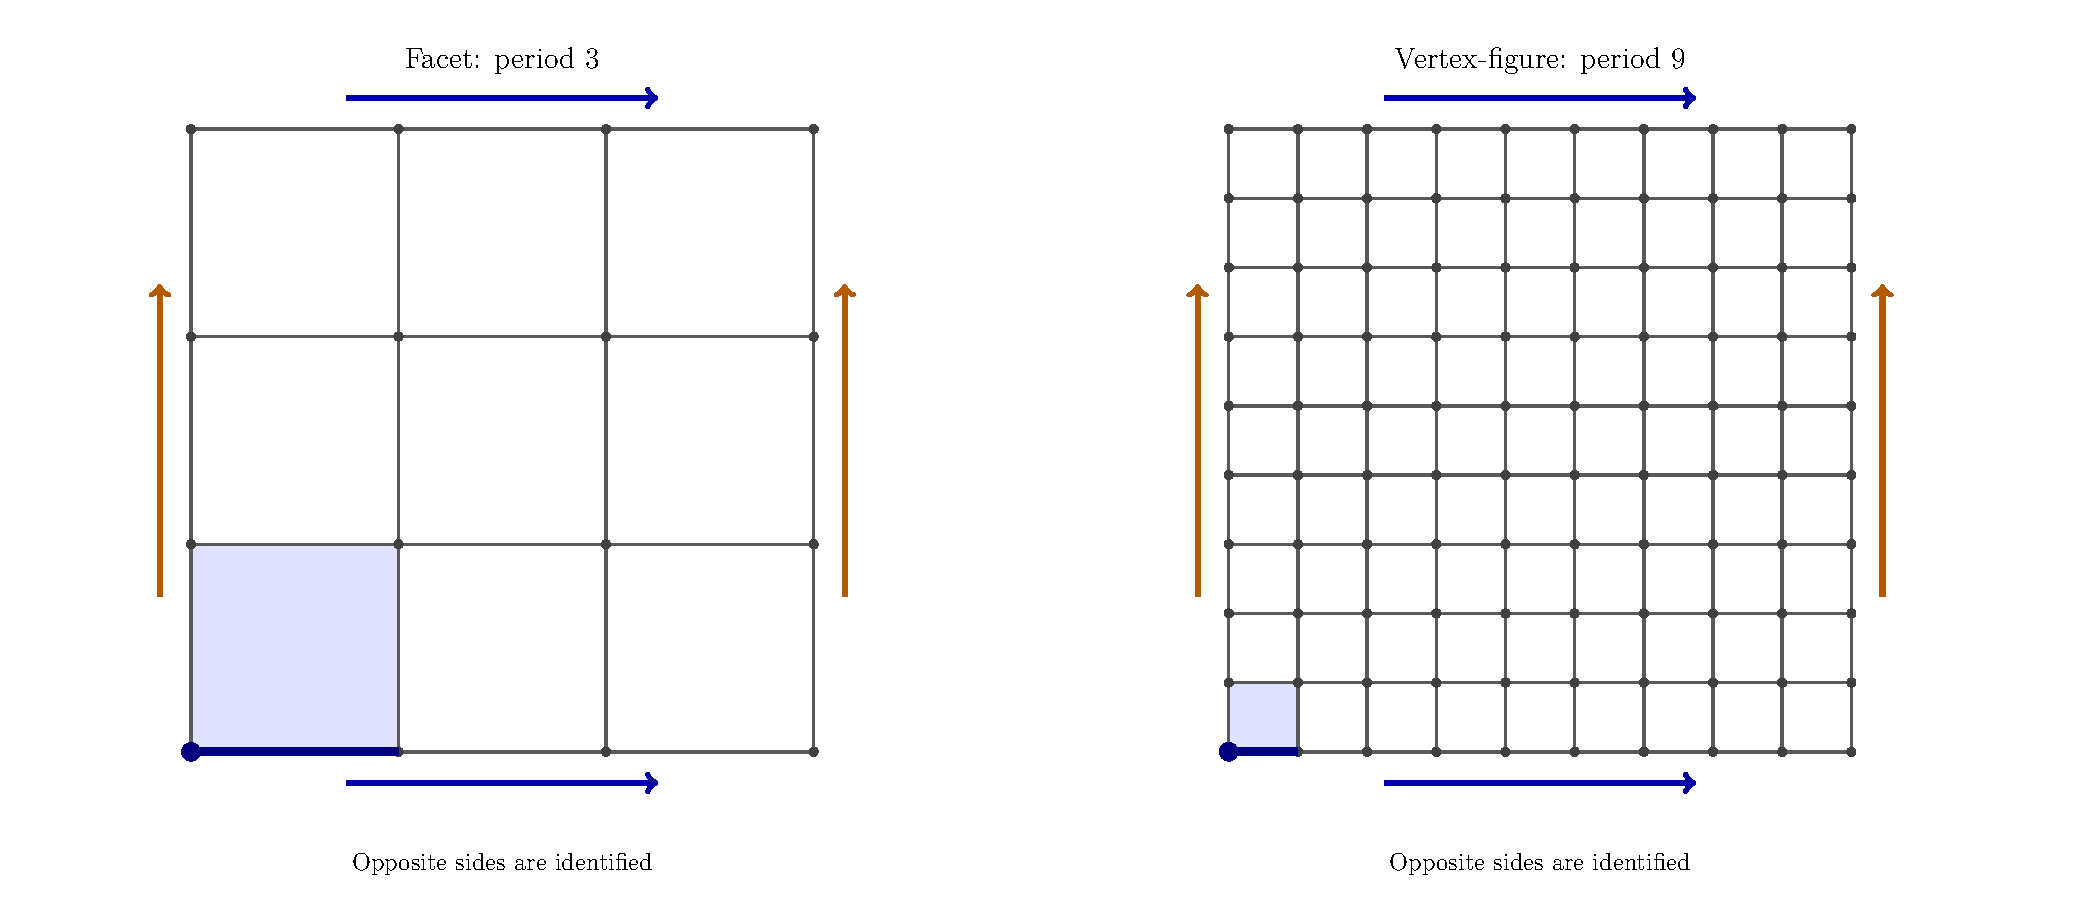
\includegraphics[width=\textwidth]{../data/local-toroids.pdf}
\caption{The facet map $\tor{3}$ and vertex-figure map $\tor{9}$ for the
$(3,9)$ instance of Theorem~\ref{thm:main}, drawn as fundamental domains
of the square tessellation. Identify the opposite sides in the directions
of the matching arrows. Boundary vertices are repeated representatives
of the same torus vertices. The shaded square, thick edge and marked
vertex form a base flag. The panels depict the two local maps of the
universal regular 4-polytope. The drawing is generated from their vertex,
edge and square data, checked against the grid-quotient definition
identified here with the coset map of $T_p$.}
\label{fig:local-maps}
\end{figure}

For a group generated by $g_0,\ldots,g_{n-1}$, put
$G_I=\ang{g_i:i\in I}$ for each subset $I$ of the index set.
An involution is a nonidentity group element whose square is the identity;
in particular, the distinguished involutions below satisfy $g_i^2=1$.
\begin{definition}\label{def:string}
A group $G=\ang{g_0,\ldots,g_{n-1}}$ with distinguished involutions is a
\emph{string C-group} if $g_i g_j=g_j g_i$ whenever $|i-j|\geq2$, and
\begin{equation}\label{eq:IP}
                  G_I\cap G_J=G_{I\cap J}
          \qquad(I,J\subseteq\{0,\ldots,n-1\}).
\end{equation}
\end{definition}
The generators of $T_p$ have this property: the square torus is a regular
polytope, and the distinguished generators of any regular polytope satisfy
the string relations and intersection property \cite[Section 2]{SW}.
Here their affine action was identified with the full torus group above.
String C-groups reconstruct regular
polytopes \cite[Theorem 2E11]{ARP}. We will use the rank-four criterion:
if the subgroups on $g_0,g_1,g_2$ and on $g_1,g_2,g_3$ are string
C-groups and meet in $\ang{g_1,g_2}$, the string relations imply
\eqref{eq:IP} for all subsets \cite[Proposition 2E16]{ARP}.

Define the universal candidate by
\begin{equation}\label{eq:Gamma}
\begin{split}
 \Gamma(s,u)=\ang{r_0,r_1,r_2,r_3\mid {}&r_i^2=1\ (0\leq i\leq3),\\
 &(r_0r_1)^4=(r_1r_2)^4=(r_2r_3)^4=1,\\
 &(r_0r_2)^2=(r_0r_3)^2=(r_1r_3)^2=1,\\
 &(r_0r_1r_2r_1)^s=(r_1r_2r_3r_2)^u=1}.
\end{split}
\end{equation}
We must prove that its local groups are $T_s,T_u$ and that it is a
string C-group;
neither conclusion follows merely by writing down the relators.

\section{An explicit matrix construction}\label{sec:matrices}
We now construct the finite image of \eqref{eq:Gamma} and calculate its
local groups. Fix distinct odd integers $s,u\geq3$ for the remainder of
the proof. All matrix entries in this section belong to a finite field
$K$ of characteristic two. The notation $\mathbf 1$ denotes the
$4\times4$ identity matrix; the letters $I,J$ in
Definition~\ref{def:string} denote index sets only.

\subsection{Parameters and generators}
We choose a common finite field and parameters encoding the two prescribed
periods, then define the four generators.
Let $k=\varphi(su)$, where $\varphi$ is Euler's totient function, and
choose $K=\F_{2^k}$. Since $su$ is odd, Euler's theorem gives
$su\mid2^k-1$. The cyclic group $K^\times$ therefore contains elements
$\lambda,\mu$ of exact orders $s,u$. Set
\begin{equation}\label{eq:parameters}
 \sigma=\lambda+\lambda^{-1},\qquad
 \tau=\mu+\mu^{-1},\qquad a=\frac{\sigma^2}{\tau},\qquad b=\sigma+a.
\end{equation}
These parameters satisfy
\begin{equation}\label{eq:nonzero}
       \sigma\tau ab\ne0,\qquad a+b=\sigma,\qquad (a+b)^2/a=\tau.
\end{equation}
Indeed, either trace is zero only if the corresponding element has
square one. Equality of the two traces would give
$(\mu-\lambda)(\mu-\lambda^{-1})=0$, contradicting their distinct
orders. Hence $b=\sigma(\tau+\sigma)/\tau$ is nonzero too.
This choice of field uses no coprimality between $s$ and $u$.

For $c\in K$ define $R(c)$, and then the four generators, by
\begin{equation}\label{eq:matrices}
\begin{gathered}
 R(c)=\begin{pmatrix}1&1&0&0\\0&1&0&0\\c&0&1&1\\0&c&0&1\end{pmatrix},
 \qquad \rho_0=R(a),\quad \rho_2=R(b),\\[3pt]
 \rho_1=\begin{pmatrix}1&0&0&0\\0&1&1&0\\0&0&1&0\\0&0&0&1\end{pmatrix},
 \qquad
 \rho_3=\begin{pmatrix}0&0&0&a^{-1}\\0&1&0&0\\0&0&1&0\\a&0&0&0\end{pmatrix}.
\end{gathered}
\end{equation}
They are invertible because their squares are $\mathbf 1$.
Put $\Lambda=\ang{\rho_0,\rho_1,\rho_2,\rho_3}\leq\GL_4(K)$.
Direct multiplication gives the string relations and the three adjacent
fourth-power relations. Each adjacent product has order exactly four:
using indices $1,2,3,4$, the $(1,1)$ entries of $(\rho_0\rho_1)^2-\mathbf 1$ and
$(\rho_1\rho_2)^2-\mathbf 1$ are $a,b$, while the $(1,2)$ entry of
$(\rho_2\rho_3)^2-\mathbf 1$ is $\sigma/a$. All three are nonzero.

\subsection{Translation orders and independent directions}
We prove that each local group has two independent translation directions
of the prescribed order. Define the translations and their subgroups by
\begin{equation}\label{eq:translations}
\begin{gathered}
 T=\rho_0\rho_1\rho_2\rho_1,\quad T'=\rho_1T\rho_1,
 \qquad V=\rho_1\rho_2\rho_3\rho_2,\quad V'=\rho_2V\rho_2,\\
 A=\ang{T,T'},\qquad B=\ang{V,V'},\qquad D=\ang{\rho_1,\rho_2},\\
 F=\ang{\rho_0,\rho_1,\rho_2},\qquad E=\ang{\rho_1,\rho_2,\rho_3}.
\end{gathered}
\end{equation}
For the fixed trace parameter $\tau$ from \eqref{eq:parameters}, put
$q_\tau(X)=X^2+\tau X+1$. Evaluating this polynomial at a matrix $M$ gives
$q_\tau(M)=M^2+\tau M+\mathbf 1$.
The polynomial $q_\tau$ is distinct notation from the reflections
$q_0,q_1,q_2$ of Section~\ref{sec:groups}.
The identities in Appendix~\ref{app:matrices}, together with the explicit
matrices there, give the calculations needed for the following proof.

\begin{lemma}\label{lem:translations}
For the matrices \eqref{eq:matrices} with parameters
\eqref{eq:parameters}, the elements $T,T'$ have order $s$, the elements
$V,V'$ have order $u$, and
\[
                       A\cong C_s\times C_s,\qquad
                       B\cong C_u\times C_u,
\]
where $C_p$ denotes a cyclic group of order $p$.
\end{lemma}
\begin{proof}
The polynomial $X^2+\sigma X+1$ has distinct roots
$\lambda,\lambda^{-1}$. The matrix $T$ is nonscalar: its $(1,3)$ entry
is one. Thus its minimal polynomial is this quadratic. It follows that
$T$ has order $s$, and conjugation gives the same order for $T'$.
Likewise $V$ is annihilated by the squarefree polynomial
\[
             (X-1)(X-\mu)(X-\mu^{-1}).
\]
Since $V\ne \mathbf 1$, its minimal polynomial has at least one of the roots
$\mu,\mu^{-1}$ as well as, possibly, 1. Its order is therefore $u$.
Conjugation gives the same order for $V'$.

To prove independence of the two facet directions, observe that
$\mathbf 1,T,T'$ are linearly independent. Indeed, the $(1,3)$, $(2,1)$ and
$(1,1)$ entries of $\alpha \mathbf 1+\beta T+\gamma T'=0$ give successively
$\gamma=\beta$, $\sigma\beta=0$ and $\alpha=0$.
Every power of $T$ belongs to $K\mathbf 1+KT$, by its quadratic relation;
similarly powers of $T'$ belong to $K\mathbf 1+KT'$.
If $T^i(T')^j=\mathbf 1$, then $T^i=(T')^{-j}$ lies in the intersection of
these two planes and is scalar. Evaluating a scalar power at both
roots gives $\lambda^i=\lambda^{-i}$. Since $s$ is odd, this forces
$s\mid i$, and then $s\mid j$. The commuting generators consequently
give $A\cong C_s\times C_s$.

For the vertex directions, put $W=q_\tau(V)$. The identities
\eqref{eq:identities} give $W\ne0$, $VW=W$ and $q_\tau(V')W=0$.
If $V^i(V')^j=\mathbf 1$, commutation implies $(V')^jW=W$.
The polynomial $q_\tau(X)$ has roots $\mu,\mu^{-1}$. If $u\nmid j$,
then $q_\tau(X)$ and $X^j-1$ are coprime. Evaluating a Bézout identity
at $V'$ and multiplying by $W$ would give $W=0$, a contradiction:
both polynomial summands annihilate $W$ by the two identities above.
Thus $u\mid j$, and the order of $V$ then gives $u\mid i$.
This proves $B\cong C_u\times C_u$.
\end{proof}

\begin{proposition}\label{prop:locals}
For the matrices \eqref{eq:matrices}, the assignments
$q_i\mapsto\rho_i$ and $q_i\mapsto\rho_{i+1}$ give isomorphisms
$T_s\cong F$ and $T_u\cong E$, respectively. Both preserve the
distinguished generators, and $|F|=8s^2$, $|E|=8u^2$.
Moreover $F=A\rtimes D$ and $E=B\rtimes D$, with $|D|=8$.
\end{proposition}
\begin{proof}
The product $\rho_1\rho_2$ has order four, so $D$ is dihedral of order
eight. The conjugation identities are
\begin{equation}\label{eq:conjugation}
\begin{array}{c|cccc}
 &T&T'&V&V'\\ \hline
 \rho_1(\cdot)\rho_1&T'&T&V^{-1}&V'\\
 \rho_2(\cdot)\rho_2&T&(T')^{-1}&V'&V
\end{array}
\end{equation}
and show that $D$ normalizes $A$ and $B$.
The identities
\[
              \rho_0=T\rho_1\rho_2\rho_1,\qquad
              \rho_3=\rho_2\rho_1V\rho_2
\]
show that $F=AD$ and $E=BD$.
The odd orders $|A|=s^2$ and $|B|=u^2$ imply $A\cap D=B\cap D=1$.
This gives the asserted orders and semidirect products.
Finally the local relations induce surjections $T_s\to F$ and
$T_u\to E$. The bound $|T_p|\leq8p^2$ from
Section~\ref{sec:groups}, together with the image orders just proved,
makes both maps isomorphisms.
\end{proof}

\section{The local intersection}\label{sec:intersection}
We prove $F\cap E=D$. The local groups have the required sizes, but
that does not by itself control their intersection. The following
commutator obstruction is the reason that shared divisors of $s$ and
$u$ cause no problem.

\begin{lemma}\label{lem:commutant}
For the matrices \eqref{eq:matrices} with parameters
\eqref{eq:parameters}, if $n\geq0$ and $T^nV=VT^n$, then $s\mid n$.
\end{lemma}
\begin{proof}
The quadratic relation for $T$ gives scalars $\alpha,\beta\in K$ with
\begin{equation}\label{eq:power}
 T^n=\alpha \mathbf 1+\beta T,\qquad
 \lambda^n=\alpha+\beta\lambda,\qquad
 \lambda^{-n}=\alpha+\beta\lambda^{-1}.
\end{equation}
These formulas follow simultaneously by induction, using
the same quadratic relation for $T,\lambda,\lambda^{-1}$.
Commuting the first formula with $V$ gives $\beta(TV-VT)=0$.
But direct multiplication gives
\begin{equation}\label{eq:commutator}
                         (TV-VT)_{12}=\sigma/a\ne0.
\end{equation}
Hence $\beta=0$. The remaining formulas in \eqref{eq:power} give
$\lambda^n=\lambda^{-n}$, so $s\mid2n$. Since $s$ is odd,
$s\mid n$, as required.
\end{proof}

\begin{lemma}\label{lem:translationintersection}
For the translation subgroups $A,B$ in \eqref{eq:translations}, with
parameters \eqref{eq:parameters}, one has $A\cap B=1$.
\end{lemma}
\begin{proof}
Let $z\in A\cap B$ and write $z=T^i(T')^j$, with $0\leq i,j<s$.
Conjugation by $\rho_2$ fixes $T$ and inverts $T'$, so
\[
 z(\rho_2z\rho_2)=T^{2i},\qquad
 z(\rho_2z\rho_2)^{-1}=(T')^{2j}.
\]
Both elements belong to $B$, since $D$ normalizes $B$.
Conjugating the second one by $\rho_1$ shows that $T^{2j}\in B$ too.
The group $B$ is abelian and contains $V$. Thus $T^{2i}$ and $T^{2j}$
commute with $V$. Lemma~\ref{lem:commutant} gives $s\mid2i$ and
$s\mid2j$. Oddness of $s$ gives $s\mid i,j$, whence $z=\mathbf 1$.
\end{proof}

\begin{proposition}\label{prop:intersection}
For the local matrix groups $F,E,D$ in \eqref{eq:translations}, with
parameters \eqref{eq:parameters}, one has
\[
                               F\cap E=D.
\]
\end{proposition}
\begin{proof}
The inclusion $D\subseteq F\cap E$ is immediate.
For the reverse inclusion, let $z\in F\cap E$. Write $z=td$ with
$t\in A$ and $d\in D$, using Proposition~\ref{prop:locals}.
Then $t=zd^{-1}\in E$. Its order is odd, because $|A|=s^2$ is odd.
But $B$ is normal in $E$, and $|E/B|=8$. The image of $t$ in $E/B$
has order dividing both eight and an odd number; it is therefore trivial.
Thus $t\in B$. Lemma~\ref{lem:translationintersection} now gives
$t=\mathbf 1$, so $z=d\in D$.
\end{proof}

This argument never compares divisors of $s$ with divisors of $u$.
The only cancellations are by two in the facet period, and by a power
of two in a quotient of the vertex-figure group. Coprimality of the two
periods is unnecessary.

The local isomorphisms of Proposition~\ref{prop:locals} and the rank-four
criterion also show that $\Lambda$ is a string C-group. Because its
matrices are over a finite field, its coset polytope is a finite regular
4-polytope with facets $\tor{s}$ and vertex-figures $\tor{u}$.
This gives a finite realization for every pair in the theorem. The next
section concerns the universal member, whose group maps onto
$\Lambda$ and need not be identified with it.

\section{The universal group and polytope}\label{sec:universal}
We transfer the intersection calculation from the finite matrix image
to the full presentation \eqref{eq:Gamma}, then recover its faces and
universal covering property.

\begin{theorem}\label{thm:group}
Let $s,u\geq3$ be distinct odd integers, and let $\Gamma(s,u)$ be the
group with exactly the presentation \eqref{eq:Gamma}.
Its distinguished generators form a string C-group, and all three
adjacent products have order exactly four. The homomorphisms from
\eqref{eq:toroid} give distinguished-generator-preserving isomorphisms
\[
 T_s\cong\ang{r_0,r_1,r_2},\qquad
 T_u\cong\ang{r_1,r_2,r_3}.
\]
These subgroups have orders $8s^2$ and $8u^2$, respectively.
\end{theorem}
\begin{proof}
The matrix relations and Lemma~\ref{lem:translations} give an epimorphism
$\pi:\Gamma(s,u)\to\Lambda$ with $\pi(r_i)=\rho_i$.
Put $\widehat F=\ang{r_0,r_1,r_2}$,
$\widehat E=\ang{r_1,r_2,r_3}$ and $\widehat D=\ang{r_1,r_2}$.
There are surjections $T_s\to\widehat F\to F$ and
$T_u\to\widehat E\to E$. The composed maps $T_s\to F$ and $T_u\to E$ are exactly the
generator-preserving isomorphisms of Proposition~\ref{prop:locals}.
Hence each map in the two chains is an isomorphism,
and $\pi$ is injective on both $\widehat F$ and $\widehat E$.
In particular, both are string C-groups with the displayed generators.

If $z\in\widehat F\cap\widehat E$, then
$\pi(z)\in F\cap E=D=\pi(\widehat D)$.
Choose $d\in\widehat D$ with $\pi(z)=\pi(d)$.
Both $z,d$ lie in $\widehat F$, where $\pi$ is injective. Thus $z=d$,
proving $\widehat F\cap\widehat E=\widehat D$.
The rank-four criterion recalled in Section~\ref{sec:groups} now
proves the intersection property for every pair of index subsets.
The string relations already hold in the presentation.
Finally the adjacent products have fourth power one in $\Gamma(s,u)$
and images of order four in $\Lambda$, so their orders are exactly four.
Each generator is consequently a nonidentity involution.
\end{proof}

\begin{proof}[Proof of Theorem~\ref{thm:main}]
Let $\Gamma=\Gamma(s,u)$. For $i=0,1,2,3$ put
$H_i=\ang{r_j:j\ne i}$. The proper faces of rank $i$ are the left
cosets $gH_i$. Two proper faces of different ranks are incident if their
cosets meet; orient this incidence by rank, and adjoin a least face of
rank $-1$ and a greatest face of rank 4. This is the coset construction
$P(\Gamma)$ of \cite[Section 2E]{ARP}. Theorem~\ref{thm:group} supplies the string C-group
hypotheses, so the construction is a regular 4-polytope.

By the reconstruction theorem \cite[Theorem 2E11]{ARP}, left multiplication
identifies $\Gamma$ with the full automorphism group, acting simply
transitively on flags.

The facets are the coset polytopes of $\widehat F$, and the
vertex-figures those of $\widehat E$.
Their generator-preserving identifications with $T_s,T_u$ show that
they are $\tor{s},\tor{u}$, with the geometric meanings established in
Section~\ref{sec:groups}. Exact adjacent orders give Schläfli type
$\{4,4,4\}$.

It remains to check universality. Let $Q$ be any regular 4-polytope
with these facets and vertex-figures, and choose a base flag.
Its distinguished involutions satisfy the Coxeter relations of
\eqref{eq:Gamma}. The two local types imply the two
additional period relations. Thus $r_i$ may be sent to the corresponding
distinguished involution of $Q$, giving a surjection
$\Gamma\to\Aut(Q)$, where $\Aut(Q)$ is the group of
order automorphisms of $Q$, meaning bijections preserving its partial order
in both directions. On cosets, this sends $gH_i$ to the image under
$g$ of the base face of rank $i$ of $Q$.
It is well-defined because every generator of $H_i$ fixes that face.
The map is surjective and preserves rank, incidence and flag adjacency,
so it is a covering. Therefore $P(\Gamma)$ is the universal member
$\{\tor{s},\tor{u}\}$, as asserted. This is the universal construction
of \cite[Theorem 4A2]{ARP} in this particular class.
\end{proof}

\section{Formalization}\label{sec:lean}
The accompanying Lean proof establishes the group and geometric polytope
conclusions from their definitions. It includes the finite-field choice,
the local orders, the full intersection property, and the transfer to the
universal presentation. The square torus is defined independently of a
group as the vertex sets of grid faces modulo $p\Z^2$, ordered by inclusion;
the proof identifies it with the local coset polytope. Regularity, the
full automorphism group, and the universal covering property are also
included.

The formal group theorem asserts the exact presentation, the full
intersection property, and the two generator-preserving local isomorphisms.
The formal geometric theorem constructs the regular polytope with the
specified square-torus sections and its covering onto every regular
polytope with those local sections.\footnote{The corresponding declarations
are \path{P16c.Main.p16c} and
\path{P16c.p16c_polytope_geometric}, respectively. Their proofs use only
\texttt{propext}, \texttt{Classical.choice} and \texttt{Quot.sound}.}
Trust rests on the Lean kernel and the stated foundational definitions.

\appendix
\section{Matrix calculations}\label{app:matrices}
We give the explicit translation matrices and collect the multiplication
identities used in Section~\ref{sec:matrices}. The notation is that of
\eqref{eq:parameters} and \eqref{eq:translations}; in particular,
$\sigma=a+b$ and $\tau=(a+b)^2/a$.
Expanding the products in \eqref{eq:translations} gives
\[
 T=\begin{pmatrix}
 1+b&0&1&1\\ b&1&0&1\\
 \sigma&\sigma&1+\sigma&0\\ ab&\sigma&b&1+a
 \end{pmatrix},\qquad
 V=\begin{pmatrix}
 0&\sigma/a&0&a^{-1}\\
 \sigma&1+\tau&1&\sigma/a\\
 \sigma&\tau&1&\sigma/a\\
 a&\sigma&0&0
 \end{pmatrix}.
\]
The quadratic expression used to separate the vertex translations is
\[
 q_\tau(V)=V^2+\tau V+\mathbf 1=
 \begin{pmatrix}
 \tau&0&\sigma/a&0\\
 \sigma&0&0&\sigma/a\\
 0&0&0&0\\
 0&0&\sigma&\tau
 \end{pmatrix}.
\]
With $T'=\rho_1T\rho_1$ and $V'=\rho_2V\rho_2$, multiplication gives
the entries $(T')_{13}=1$, $(T')_{21}=a$ and $(T')_{11}=1+b$ used to
check independence in Lemma~\ref{lem:translations}, and the identities
\begin{equation}\label{eq:identities}
\begin{gathered}
 T^2=\sigma T+\mathbf 1,\qquad (T')^2=\sigma T'+\mathbf 1,\qquad TT'=T'T,\\
 VV'=V'V,\qquad (V+\mathbf 1)q_\tau(V)=0,\qquad
                   (V'+\mathbf 1)q_\tau(V')=0,\\
 q_\tau(V')q_\tau(V)=0,\qquad (q_\tau(V))_{11}=\tau,\qquad V\ne \mathbf 1.
\end{gathered}
\end{equation}
These are identities in characteristic two with the parameter relations
\eqref{eq:nonzero}. The displayed matrices exhibit $T_{13}=1$,
$V_{11}=0$ and $(q_\tau(V))_{11}=\tau\ne0$, which are the nonvanishing
entries used in Lemma~\ref{lem:translations}.

\begin{thebibliography}{99}
\bibitem{CM}
H.~S.~M. Coxeter and W.~O.~J. Moser,
\emph{Generators and Relations for Discrete Groups}, 4th ed.,
Ergebnisse der Mathematik und ihrer Grenzgebiete 14, Springer, 1980.

\bibitem{FPmaps}
M.~E. Fernandes and C.~A. Piedade,
\emph{Faithful permutation representations of toroidal regular maps},
J. Algebraic Combin. \textbf{52} (2020), 317--337.
\href{https://doi.org/10.1007/s10801-019-00904-8}{doi:10.1007/s10801-019-00904-8};
\href{https://arxiv.org/abs/1808.09705}{arXiv:1808.09705}.
Correction: J. Algebraic Combin. \textbf{54} (2021), 733--738,
\href{https://doi.org/10.1007/s10801-020-00985-w}{doi:10.1007/s10801-020-00985-w}.

\bibitem{FPdegrees}
M.~E. Fernandes and C.~A. Piedade,
\emph{The degrees of regular polytopes of type $[4,4,4]$},
SIAM J. Discrete Math. \textbf{36} (2022), 1143--1155.
\href{https://doi.org/10.1137/20M1375012}{doi:10.1137/20M1375012}.

\bibitem{MS92}
P.~McMullen and E.~Schulte,
\emph{Regular polytopes of type $\{4,4,3\}$ and $\{4,4,4\}$},
Combinatorica \textbf{12} (1992), 203--220.
\href{https://doi.org/10.1007/BF01204723}{doi:10.1007/BF01204723}.

\bibitem{ARP}
P.~McMullen and E.~Schulte,
\emph{Abstract Regular Polytopes}, Encyclopedia of Mathematics and its
Applications 92, Cambridge University Press, 2002.
\href{https://doi.org/10.1017/CBO9780511546686}{doi:10.1017/CBO9780511546686}.

\bibitem{MonS}
B.~Monson and E.~Schulte,
\emph{Reflection groups and polytopes over finite fields, II},
Adv. Appl. Math. \textbf{38} (2007), 327--356.
\href{https://doi.org/10.1016/j.aam.2005.12.001}{doi:10.1016/j.aam.2005.12.001};
\href{https://arxiv.org/abs/math/0601502}{arXiv:math/0601502}.

\bibitem{CFH}
M.~D.~E. Conder, Y.-Q. Feng and D.-D. Hou,
\emph{Two infinite families of chiral polytopes of type
$\{4,4,4\}$ with solvable automorphism groups},
\href{https://doi.org/10.1016/j.jalgebra.2020.11.002}{doi:10.1016/j.jalgebra.2020.11.002};
\href{https://arxiv.org/abs/1912.03398}{arXiv:1912.03398}.

\bibitem{CFHS}
G.~Cunningham, Y.-Q. Feng, D.-D. Hou and E.~Schulte,
\emph{Symmetric polytopes whose automorphism groups are 2-groups},
\href{https://doi.org/10.1016/j.jalgebra.2026.03.017}{doi:10.1016/j.jalgebra.2026.03.017};
\href{https://arxiv.org/abs/2512.15511}{arXiv:2512.15511}.

\bibitem{CH}
G.~Cunningham and I.~Hubard,
\emph{Polytopality criteria for the mix of polytopes and maniplexes},
\href{https://arxiv.org/abs/2506.19334}{arXiv:2506.19334}.

\bibitem{SW}
E.~Schulte and A.~Ivi\'c Weiss,
\emph{Problems on polytopes, their groups, and realizations},
Period. Math. Hungar. \textbf{53} (2006), 231--255.
\href{https://doi.org/10.1007/s10998-006-0035-y}{doi:10.1007/s10998-006-0035-y};
\href{https://arxiv.org/abs/math/0608397}{arXiv:math/0608397}.
\end{thebibliography}
\end{document}
